\section{Technical Overview}\label{sec:tech-overview}
As we have alluded to earlier, existing memory-checking based techniques to model RAM computations incur a cost
that is linear in the size of the RAM. We are interested in the setting where the number of operations whose
execution is to be verified is much smaller than the size of the RAM. Thus, our goal is to achieve prover complexity
which is {\em sublinear} in the size of the RAM. Before we proceed, we establish a
working definition of RAM for the rest of the paper. Informally, a RAM maps indices (addresses) to values, where
we assume that values come from a finite field $\F$, while indices come from a subset $\setind$ of $\F$. For us,
$\setind$ will generally be the set $\{1,\ldots,k\}$ for some integer $k$ (which may be different from size of
the RAM $n$). Finally, for an index, there should be at most one value in the RAM, i.e., the association is unambiguous.
The formal definition of the RAM follows:
\begin{definition}[RAM]\label{defn:RAM}
Given $n\in \N$, finite field $\F$ and a set $\mathcal{I}\subseteq \F$, a RAM of size $n$ over indices $\mathcal{I}$
is a tuple $T=(\vec{a},\vec{v})\in \mathcal{I}^n\times \F^n$ such that $\forall\, i,j\in [n]$  $v_i=v_j$ whenever $a_i=a_j$.
We think of $T$ as a table with vectors $\vec{a}$ and $\vec{v}$ denoting its columns. The set of all such
tables will be denoted by $\RAM{I}{n}$.
    %\begin{align*}
    %        T[\,a\,] = \begin{cases}
    %                   v \text{ if } \, \exists i\in [n] \text{ s.t. } (a,v) = (a_i,v_i), \\
    %                  \bot \text{ otherwise }
    %                \end{cases}
    %\end{align*}
\end{definition}
For a table $T=(\vec{a},\vec{v})\in \RAM{I}{n}$, we refer to tuples $(a_i,v_i)$, $i\in [n]$ as records of the table $T$.
We use the access notation $v=T[a]$ to mean that $(a,v)$ is a record of $T$ (note there can be multiple such records
according to our definition). When we refer to a vector $\vecT\in \F^n$ as a RAM, we implicitly
assume $T=(\setind_n,\vecT)$ with $\setind_n=(1,2,\ldots,n)$. In this case we have $T[i]=\vecT[i]$.
For a RAM $T\in \RAM{I}{n}$, a RAM operation is a three tuple $(\op,a,v)$ with $\op\in \{0,1\}$,
$a\in \setind$ and $v\in \F$. An operation with $\op=0$ is called a {\em load} operation which denotes reading a value $v$
mapped to index $a$ in the RAM. Similarly, an operation with $\op=1$ is called a {\em store} operation,
which denotes associating the value $v$ with index $a$ in the RAM.
We use $\RAMOp{I}$ to denote the set of all RAM operations with index set $\setind$.

\begin{table*}[bt]
    \begin{tabular}{l|l|l|l|l}
        \hline
        {\bf Component  }                                                                                      & {\bf Protocol} & {\bf Prover Work}      & {\bf Verifier Work} & {\bf Communication}   \\ \hline
        Committed Sub-vector Lookup                                                                     & CQ ~\cite{EPRINT:EagFioGab22}      & $O(m \log m)\,\F$, $O(m)\,\Gone$      & 5P            & $8\Gone$, $3\F$         \\ \hline
        Committed Index Lookup                                                                          & Fig ~\ref{fig:committed-index-lookup}    & $O(m \log m)\,F$, $O(m)\,\Gone$      & 5P            & $8\Gone$, $3\F$         \\ \hline
        Localized Update in RAM                                                                                & Fig ~\ref{fig:a-identical}   & $O(m \log^2 m)\, \F$, $O(m)\,\Gone$      & 7P            & $19\Gone$, $1\Gtwo$, $10\F$ \\ \hline
        Table Specific Preprocessing                                                                    & Fast KZG ~\cite{EPRINT:FeiKho23}      & $O(N \log N)\,\F,\G$      & -             & -               \\ \hline
        Lookup from Approximate Setup                                                                   & Sec ~\ref{sec:update-protocol}    & $O((m+\delta)\log^2(m+\delta))\,\F$, $O(m+\delta)\,\Gone$ & -             & -               \\ \hline
        Polynomial Protocol for RAM                                                                     & Fig ~\ref{fig:covering-protocol}   & $O(m \log m)\, \F,\G$      & 6P            & $36\Gone$, $30\F$       \\ \hline
        %	Concatenation of transcripts                                                                    & Fig 8    & $O(m \log m)$      & 2P            & 4G1, 6F         \\ \hline
        %	Permutation of transcripts                                                                      & Fig 9    & $O(m \log m)$       & 2P            & 4G1, 5F         \\ \hline
        %	\begin{tabular}[c]{@{}l@{}}Memory consistency \& \\ address ordering of transcript\end{tabular} & Fig 7    & $O(m \log m)$       & 5P            & 20G1,19F        \\ \hline
        \rowcolor{gray}
        Batching-Efficient RAM                                                                          & Fig  ~\ref{fig:complete-listing}    & $\widetilde{O}(\sqrt{mN})\,\F,\G$            & 8P            & $65\Gone$, $1\Gtwo$, $43\F$  \\ \hline
    \end{tabular}
    \caption{Asymptotic Efficiency of Component Protocols. Here $N$ = size of the RAM, $m$ = number of operations
    , $\delta$ = hamming distance of table for which pre-computed parameters are available from the current table.
    $P$ denotes a pairing evaluation. The performance corresponds to CQ based realization of batching-efficient
    RAM.}
    \label{tbl:efficiency-components}
\end{table*}



\subsection{Batching-Efficient RAM: Blueprint}\label{subsec:batching-efficient-ram-blueprint}
We will use a vectors in $\F^N$ to denote the ``large'' RAMs, where index column is implicitly
assumed to be $(1,\ldots,N)$.
Let $\vec{T},\vec{T'}\in \F^N$ denote the initial and final RAM states, and let $\vec{o}$ be
a sequence of $m$ operations ($m < N$) which updates $\vec{T}$ to $\vec{T}'$. Let $\vec{a}\in \F^m$ denote the vector
of RAM indices referenced by the operations in $\vec{o}$, i.e, $a_i$ is the index referenced by $i^{th}$ operation.
To prove the transformation of $\vec{T}$ to $\vec{T}'$ via operation sequence $\vec{o}$, we proceed as follows:
\begin{itemize}[leftmargin=1em, label=-]
    \item We isolate sub-tables $S=(\vec{a},\vec{v})$ and $S'=(\vec{a},\vec{a'})$ of $T$ and $T'$ consisting of
    rows corresponding to indices in $\vec{a}$. This requires proving $\vec{v}=\vecT[\vec{a}]$ and $\vec{v'}=
    \vecT'[\vec{a}]$, which we show using {\em committed index lookup} argument discussed in Section ~\ref{subsec:committed-index-lookup}.

    \item On the isolated sub-table $S$ and $S'$ of size $m$, we use the standard memory checking arguments (c.f. argument
    presented in Section \ref{sec:poly-proto-ram-app}) to prove that sequence $\vec{o}$ correctly updates $S$ to $S'$ with
    prover complexity of $\wt{O}(m)$.

    \item Finally, we show that the RAMs $T$ and $T'$ are identical outside indices in $\vec{a}$. We describe the protocol
    for proving the same in Section ~\ref{subsec:proximity-ram}.
\end{itemize}

\begin{figure}[htbp]
    \centering
    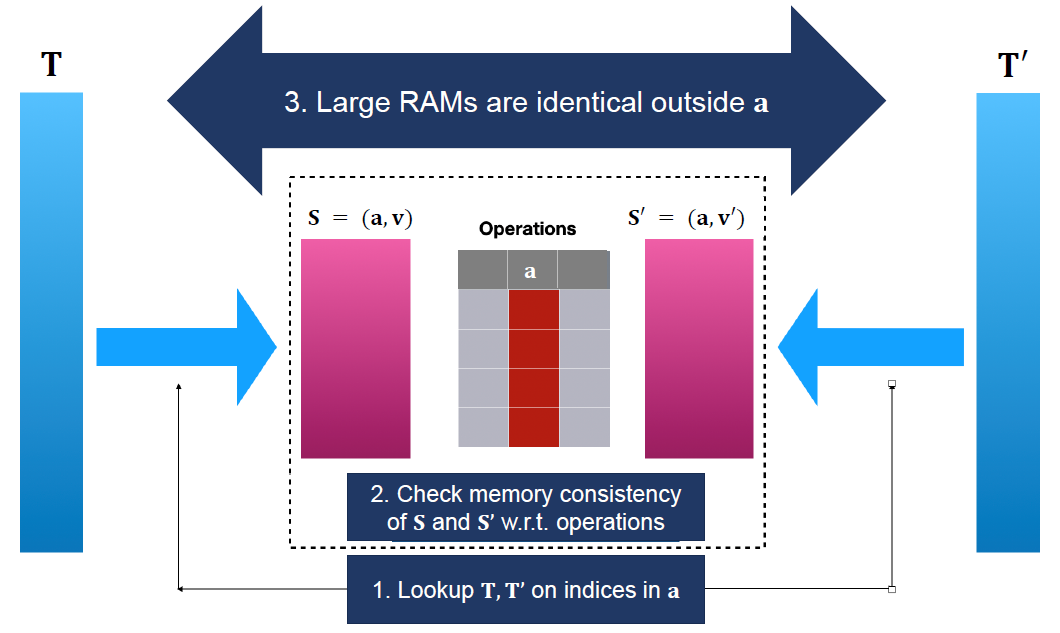
\includegraphics[width=0.4\textwidth]{RAM-Lookup}
    \caption{Illustrating different steps of sub-linear lookup protocol between large RAMs $\vecT$ and $\vecT'$.}
    \label{fig:blueprint}
\end{figure}

The blueprint for the above approach is illustrated in Figure ~\ref{fig:blueprint}.

\subsection{Batching-Efficient RAM: Components}\label{subsec:batching-efficient-ram-components}
We now elaborate on the key technical components in realizing the above blueprint.

\smallskip

\noindent{\bf Committed Index Lookup.} To limit the size of the RAM on which we use memory-checking techniques,
our first step is to isolate sub-tables of RAMs $\vecT$ and
$\vecT'$ which are actually referenced by operations. This is accomplished by looking up RAMs $\vecT$ and
$\vecT'$ at indices in the committed vector $\vec{a}$. Here, we leverage the recent work on efficient lookup
arguments to verifiably extract $m$ indices from a table of size $N$, in time dependent only on $m$.
There are two technical challenges here. First, the aforementioned lookup arguments only prove the sub-vector
relation, without linking the extracted vector to the indices in $\vec{a}$. This is easily solved, as there
is an efficient realization of a {\em committed index lookup} from a {\em committed sub-vector} argument,
where commitment scheme is homo-morphic. The details appear in Section ~\ref{subsec:committed-index-lookup},
with complete protocol presented in Figure ~\ref{fig:committed-index-lookup}. Second challenge is much more
formidable: the efficiency of sub-vector arguments (and the committed index lookup argument derived from them)
depends on {\em expensive} table-specific pre-processing. This is acceptable when the table in question is
static, but is infeasible in our setting requiring updatable tables. This motivates our next technical
component.

\smallskip

\noindent{\bf Fast Lookup from Approximate Setup.} We build upon the rich body of work on polynomial protocols enabling efficient lookups from static tables~\cite{CCS:ZBKMNS22,EPRINT:PosKat22,EPRINT:ZGKMR22,EPRINT:EagFioGab22}, which rely on expensive table-dependent pre-computation
to optimise online proving performance. We make the first attempt towards breaking this rigid dependence.
Our key idea is to extend the utility of pre-computed
parameters for a table $\vecT$, to proving lookups from tables $\vecT'\neq \vecT$.
We show that for $\delta=\Delta(\vecT, \vecT')$,
an argument for $m$ lookups from $\vecT'$ incurs an additional prover overhead of $(m+\delta)\log^2(m+\delta)$ over the
lookup argument for static tables. We note that overhead is {\em quasi}-linear in both $m$ and $\delta$.
Our competitive overhead rests on several innovative applications of algebraic
algorithms, which are summarised in Section ~\ref{subsec:comp-algebra-app}. We then leverage this ability to use ``approximate"
setup into a {\em base + cache} strategy; where at all times we maintain pre-computed parameters corresponding to
a base table $\vecTbase$, and use this setup to prove lookups from the current table $\vecT$. We achieve optimal
prover effort on average by using parameters for $\vecTbase$ till the current table is at a hamming distance
at most $\sqrt{mN}$ from $\vecTbase$, beyond which we recompute full parameters for the current table with
$O(N\log N)$ prover effort. The cycle then repeats with current table as the base table.

\smallskip

\noindent{\bf Naive Approaches are Inadequate.} We notice that the aforementioned constructions of lookup arguments require linear combination of
encoded quotients of the form $\gany{(T(X)-T(\xi^i))/(X-\xi^i)}$ for upto $m$ values of $i$ during the proof generation.
While constructions ~\cite{CCS:ZBKMNS22,EPRINT:PosKat22}
consider quotients encoded in the group $\Gtwo$, the protocol in ~\cite{EPRINT:EagFioGab22} encodes them in $\Gone$.
We use a generic $[\,\cdot\,]_g$ to
account for protocol-specific choices. We also see that even a small change to the table requires one to update all the quotients (the polynomial $T(X)$ is
common to all quotients). Updating the $|\vecT|$ quotients for each batch is clearly infeasible. One could consider delaying the updation of the quotients, till
the time they are actually required in a proof, which happens when the corresponding index in the table is involved in lookup. However, each of the $m$ quotients
is now potentially ``lagging'' by $\delta$ updates, so we would need $\Omega(m\delta)$ group operations to refresh all of them. This gives us multiplicative degradation
with $\delta$, and is clearly unsustainable for reasonable values of $\delta$. In Section ~\ref{sec:update-protocol}, we present an efficient method
to directly compute linear combination of upto $O(m)$ encoded quotients of the form $\gany{(T(X)-T(\xi^i))/(X-\xi^i)}$.

\smallskip

\noindent{\bf Localizing changes in RAMs.} While the above two components allow us to reliably extract sub-RAMs
corresponding to indices in vector $\vec{a}$, we still need to prove that RAMs are identical outside indices in
$\vec{a}$. Looking ahead, in terms of polynomials this requires proving that $T(\xi^i)=T'(\xi^i)$ for $i\not\in
\{a_i:i\in [m]\}$. Assuming $Z_I(X)$ to be the vanishing polynomial of the set $\{\xi^{a_i}:i\in [m]\}$,
this is equivalent to proving that $Z_I(X)(T(X) - T'(X)) = D(X)\vpolyN(X)$ for some polynomial $D$. However, naively
this involves working with polynomials with degree $O(N)$, which is expensive.
In Section ~\ref{subsec:proximity-ram} we show a polynomial protocol for the above relation which requires only $O(m\log^2 m)$ prover effort. The protocol
appears in Figure ~\ref{fig:a-identical}.

\smallskip

\noindent{\bf Polynomial Protocol for Memory Checking.} To complete the verification, we need to show that
the smaller RAMs, $S=(\vec{a},\vec{v})$ and $S'=(\vec{a},\vec{v}')$ extracted from larger RAMs $\vecT,\vecT'$
are consistent with respect to the operations. This can be accomplished using standard memory checking techniques
based on address ordered transcripts, which we formalize in Section ~\ref{sec:poly-proto-ram}. Later in
Section ~\ref{sec:poly-proto-ram-app}, we assemble known techniques to present a polynomial protocol
for memory consistency based on address ordered transcripts.
This involves encoding several artefacts such as operations, transcripts etc., as polynomials and relations
among them such as concatenation, permutation and monotonicity as polynomial identities. Our modelling is
simple and implementation friendly, and helps in realizing a ``circuit-free'' overall construction. Complete
polynomial protocol for memory checking appears in Figure ~\ref{fig:covering-protocol}, while constituent protocols
appear in Figures ~\ref{fig:time-ordered-transcript}, ~\ref{fig:encoded-relations} and ~\ref{fig:permutated-transcripts}.

\smallskip

\noindent{\bf Efficiency.} We conclude the overview with a discussion of efficiency achieved by our scheme, and
how different components discussed in this section contribute to the overall efficiency. The asymptotic performance
of our scheme using CQ ~\cite{EPRINT:EagFioGab22} is summarized in Table ~\ref{tbl:efficiency-components}, with
efficiency of the overall scheme highlighted in gray. The table also serves as a ready-reckoner for component protocols
involved in the overall scheme. We note that the verification complexity of the overall solution is substantially
less than the aggregate of component protocols; this is due to the fact that several pairing checks required for
$\kzg$ verification proofs can be batched together. For concrete instantiation using BLS12-381 curve, RAM size
of 1 million, the online cost of proving an update of 1000 operations on a table as a function of its
hamming distance from the ``pre-processed'' table is described in Figure ~\ref{fig:batch-ram-proving-time}.
Other performance metrics for the same setting are summarized below:
\begin{table}[htbp]
\begin{tabularx}{0.45\textwidth}{|X|X|}
\hline
{\bf Metric} & {\bf Performance} \\ \hline
Parameter Re-computation & 12000 secs \\ \hline
Verification Time & $\approx$ 10 ms \\ \hline
Argument Size & $\approx$ 4.4 KB \\
\hline
\end{tabularx}
\end{table}

Clearly, the (offline) parameter re-computation is the most expensive operation. Parallel implementations can
substantially speed up parameter re-computation as their cost is dominated by FFTs over group polynomials, which
are highly parallelizable.

\smallskip

\noindent{\bf Liveliness.} To maintain {\em liveliness} of the system in scenarios such as rollups, we must carefully
align the online prover performance curve with the cost of offline computation. As an example, suppose $\vec{T}_0$
is the initial pre-processed table at time $t=0$. We generate proofs using pre-computed parameters for $\vec{T}_0$
till the time $t=t_1$, when the table state $\vec{T}_1$ is at hamming distance $2^{17}$ from $\vec{T}_0$. At this point,
from Figure ~\ref{fig:batch-ram-proving-time}, online proof generation takes around $40s$ for batch of $1000$ updates.
At $t=t_1$, we also start an offline parameter computation for the table $\vec{T}_1$, while continuing to generate
online proofs using parameters for $\vec{T}_0$. We can generate the next $2^7$ batches of updates at an average of
approximately $12000/128\approx 94s$ each, thus finishing with a table state $\vec{T}_2$ at hamming distance at most
$2^{18}$ from $\vec{T}_0$ at $t_2=t_1+12000$. At this point, we should have the pre-computed parameters for $\vec{T}_1$,
which is at update distance of $2^{17}$ from $\vec{T}_2$, and thus online proof generation can switch to parameters
for the table $\vec{T}_1$. This alignment gives us a proving time of $94s$ per batch of $1000$, while ensuring system
is live at all times. Clearly, a faster offline pre-computation using parallel implementation would allow us to stay
at the cheaper end of online proving performance.






%which as seen earlier is given by the summation below:
%\begin{equation}\label{eq:encoded-quotient}
%\gany{\frac{T(X)-T_I(X)}{Z_I(X)}} = \sum_{i\in I}\frac{1}{Z_I'(\xi^i)}\gany{\frac{T(X)-T(\xi^i)}{X-\xi^i}}
%\end{equation}
%We now describe our approach.







%The efficiency of the above approach relies crucially on the efficiency of committed index lookup used to
%reduce the size of the RAMs for quasi-linear memory checking methods. It is tempting to use the recent lookup arguments
%in ~\cite{CCS:ZBKMNS22,EPRINT:PosKat22,EPRINT:EagFioGab22} to prove the correctness of the first step with prover complexity dependent only on $m$.
%However, employing them directly is difficult; their table-independent efficiency relies on
%table specific expensive pre-computation, which does not help when the table is updatable. This is the problem we solve
%in Section ~\ref{sec:update-protocol}, where we modify the prover algorithm for the lookup arguments to remain efficient
%with access to pre-computed parameters for an ``approximate'' table.

